% !TEX encoding = UTF-8 Unicode

% Compilation using 'acmsmall.cls' - version 1.3 (March 2012), Aptara Inc.
% (c) 2010 Association for Computing Machinery (ACM)
%
% Questions/Suggestions/Feedback should be addressed to => "acmtexsupport@aptaracorp.com".
% Users can also go through the FAQs available on the journal's submission webpage.
%
% Steps to compile: latex, bibtex, latex latex


\documentclass[prodmode,acmtecs]{acmsmall} % Aptara syntax

% Package to generate and customize Algorithm as per ACM style
\usepackage[ruled]{algorithm2e}
\renewcommand{\algorithmcfname}{ALGORITHM}
\SetAlFnt{\small}
\SetAlCapFnt{\small}
\SetAlCapNameFnt{\small}
\SetAlCapHSkip{0pt}
\IncMargin{-\parindent}

% Metadata Information
\acmVolume{9}
\acmNumber{4}
\acmArticle{39}
\acmYear{2010}
\acmMonth{3}

% Copyright
%\setcopyright{acmcopyright}
%\setcopyright{acmlicensed}
%\setcopyright{rightsretained}
%\setcopyright{usgov}
%\setcopyright{usgovmixed}
%\setcopyright{cagov}
%\setcopyright{cagovmixed}

% DOI
\doi{0000001.0000001}

%ISSN
\issn{1234-56789}

% Document starts
\begin{document}

% Page heads
\markboth{B. Harmon et al.}{Embodied Spatial Cognition in Tangible Computing}

% Title portion
\title{Embodied Spatial Cognition in Tangible Computing}
\author{BRENDAN ALEXANDER HARMON
\affil{North Carolina State University}
ANNA PETRASOVA
\affil{North Carolina State University}
VACLAV PETRAS
\affil{North Carolina State University}
HELENA MITASOVA
\affil{North Carolina State University}
ROSS MEENTEMEYER
\affil{North Carolina State University}}

\begin{abstract}
\ldots
\end{abstract}

%
% The code below should be generated by the tool at
% http://dl.acm.org/ccs.cfm
% Please copy and paste the code instead of the example below. 
%
\begin{CCSXML}
<ccs2012>
<concept>
<concept_id>10003120.10003121</concept_id>
<concept_desc>Human-centered computing~Human computer interaction (HCI)</concept_desc>
<concept_significance>500</concept_significance>
</concept>
<concept>
<concept_id>10003120.10003121.10003122.10011749</concept_id>
<concept_desc>Human-centered computing~Laboratory experiments</concept_desc>
<concept_significance>500</concept_significance>
</concept>
</ccs2012>
\end{CCSXML}

\ccsdesc[500]{Human-centered computing~Human computer interaction (HCI)}
\ccsdesc[500]{Human-centered computing~Laboratory experiments}
%
% End generated code
%

\keywords{Wireless sensor networks, media access control,
multi-channel, radio interference, time synchronization}

\acmformat{Brendan A. Harmon, Anna Petrasova, Vaclav Petras, Helena Mitasova, and Ross K. Meentemeyer, 2016. Embodied Spatial Cognition in Tangible Computing.}
% At a minimum you need to supply the author names, year and a title.
% IMPORTANT:
% Full first names whenever they are known, surname last, followed by a period.
% In the case of two authors, 'and' is placed between them.
% In the case of three or more authors, the serial comma is used, that is, all author names
% except the last one but including the penultimate author's name are followed by a comma,
% and then 'and' is placed before the final author's name.
% If only first and middle initials are known, then each initial
% is followed by a period and they are separated by a space.
% The remaining information (journal title, volume, article number, date, etc.) is 'auto-generated'.

\begin{bottomstuff}
%This work is supported by the National Science Foundation, under grant...
%
Author's addresses: B. A. Harmon {and} A. Petrasova {and} V. Petras {and} H. Mitasova {and} R. K. Meentemeyer, Center for Geospatial Analytics, North Carolina State University.
% ; G. H. Bressler, Department of Landscape Architecture, North Carolina State University.
\end{bottomstuff}

\maketitle


\section{Introduction}

% Theory

% A brief history of tangible computing

\section{Methodology}

\subsection{Tangible Landscape}

% Design

Figure~\ref{fig:system_schema} \ldots 
% Figure
\begin{figure}
\centerline{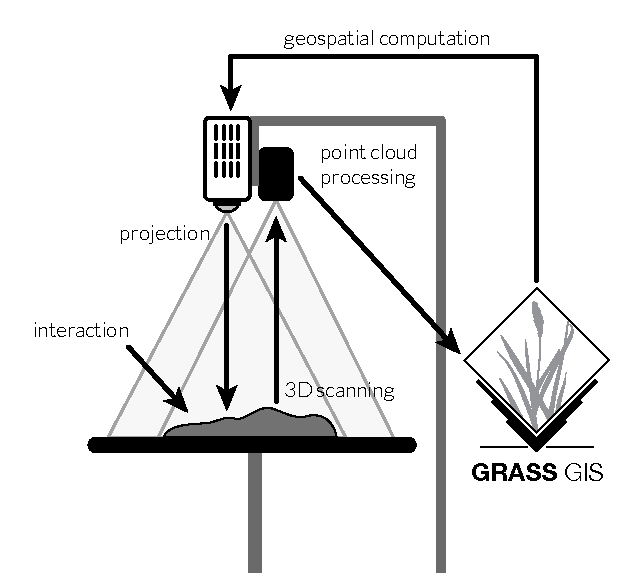
\includegraphics{images/system_schema.png}}
\caption{Caption.}
\label{fig:system_schema}
\end{figure}

% 

% Modes of interaction

% Applications


\subsection{Terrain modeling experiment}

\section{Results}

\section{Discussion}

\section{Future work}

\section{Conclusion}

%\section{...}
%% label
%\label{sec:examples}
%
%% Head 2
%\subsection{Head 2}
%
%% Head 3
%\subsubsection{Head 3}
%
%% Head 4
%\paragraph{Head 4}
%
%% quote
%\begin{quote}
%``\ldots".
%\end{quote}
%
%% itemize
%\begin{itemize}
%\item \ldots .
%\item \ldots .
%\item \ldots .
%\end{itemize}
%
%% footnote
%\ldots \footnote{...} 
%
%% enumerate
%\begin{enumerate}
%\item \ldots .
%\item \ldots . 
%\item \ldots .
%      \begin{enumerate}
%      \item \ldots .
%      \item \ldots .
%      \end{enumerate}
%\end{enumerate}
%
%% Enunciations
%\begin{definition}[...]...
%\end{definition}
%
%Table~\ref{tab:one}. 
%% Table
%\begin{table}%
%\tbl{...\label{tab:one}}{%
%\begin{tabular}{|l|l|}
%\hline
%...   & ...\\\hline
%...    & ...\\\hline
%\end{tabular}}
%\end{table}%

% Appendix
\appendix
\section*{APPENDIX}
\setcounter{section}{1}
In this appendix \ldots
\appendixhead{HARMON}

% Acknowledgments
\begin{acks}
\ldots
\end{acks}

% Bibliography
\bibliographystyle{ACM-Reference-Format-Journals}
\bibliography{tangible_topography.bib}

% History dates
%\received{}{}{}

% Electronic Appendix
\elecappendix

\medskip

\section{...}

\ldots

\end{document}



